\chapter{Detalles de implementación y experimentos}\label{chapter:implementation}

-----------------------------------------------------------------------------------
\section{Resultados}\label{sec:results}
%-----------------------------------------------------------------------------------
Tras la implementación del modelo, los resultados obtenidos de este modelo de aprendizaje automático son muy útiles y eficientes en el campo de la detección de melanomas. Con una eficacia de validación cercana al 78,9\%, el modelo es capaz de detectar la presencia de melanoma con una precisión razonable. Los resultados son un paso significativo hacia la automatización del diagnóstico del cáncer de piel, que tradicionalmente ha dependido de la inspección visual por parte de expertos humanos.

La eficacia del modelo también puede mejorarse aún más optimizando su consumo de tiempo y memoria. Esta optimización será esencial para convertir los resultados del modelo en una solución a gran escala que pueda ser utilizada por profesionales sanitarios y pacientes de todo el mundo. Es importante señalar que el entrenamiento inicial del modelo es un proceso que se realiza una sola vez y no necesita ejecutarse continuamente. Por lo tanto, si se optimiza el proceso de entrenamiento, la eficacia del modelo puede mejorar considerablemente.

%-----------------------------------------------------------------------------------
	\subsection{Estadísticas básicas}\label{sub:basic_statistics}
%-----------------------------------------------------------------------------------
    
    Estos resultados de la tabla siguiente corresponden a la evaluación del modelo a lo largo de 40 epochs (o iteraciones) de entrenamiento. Cada fila representa una época y se presentan las siguientes métricas:
    
    \begin{description}
       \item [loss:] Es una medida de la diferencia entre las predicciones del modelo y los valores reales de los datos de entrenamiento en esa época. El objetivo del entrenamiento es minimizar esta métrica.
       \item [acc (accuracy):] Es la proporción de predicciones correctas realizadas por el modelo sobre el conjunto de datos de entrenamiento en esa época.
       \item [v loss (vl) (pérdida de validación):] Es la pérdida en el conjunto de datos de validación, que es un conjunto de datos independiente que no se utiliza para entrenar el modelo, sino para evaluar su generalizabilidad.
       \item [v acc (precisión de validación):] Es la precisión en el conjunto de datos de validación.
    \end{description}
\begin{figure}[ht]
        \small
        \begin{center}
            \begin{tabular}{|c|c|c|c|c|c|c|c|} \hline
            E  & Loss  & Acc & V loss & V acc & LR             & M & Batch \\ \hline
            1  & 9.535 & 37.735   & 9.396  & 38.4  & $10^{-2}$ & Acc     & 1337.97 \\ \hline
            2  & 7.791 & 66.306   & 7.832  & 61.6  & $10^{-2}$ & Acc     & 414.44 \\ \hline
            3  & 6.852 & 79.624   & 7.042  & 66.8  & $10^{-2}$ & Acc     & 291.03 \\ \hline
            4  & 6.191 & 85.544   & 6.398  & 67.6  & $10^{-2}$ & Acc     & 281.46 \\ \hline
            5  & 5.594 & 90.894   & 5.772  & 72.8  & $10^{-2}$ & Acc     & 288.00 \\ \hline
            6  & 5.111 & 92.943   & 5.311  & 74.4  & $10^{-2}$ & Vl  & 280.35 \\ \hline
            7  & 4.653 & 95.788   & 4.916  & 74.4  & $10^{-2}$ & Vl  & 274.80 \\ \hline
            8  & 4.268 & 95.788   & 4.631  & 73.6  & $10^{-2}$ & Vl  & 280.88 \\ \hline
            9  & 3.888 & 97.097   & 4.164  & 76.8  & $10^{-2}$ & Vl  & 302.48 \\ \hline
            10 & 3.547 & 97.553   & 3.840  & 76.4  & $10^{-2}$ & Vl  & 275.76 \\ \hline
            11 & 3.233 & 98.349   & 3.622  & 75.2  & $10^{-2}$ & Vl  & 281.52 \\ \hline
            \dots   & \dots   & \dots      & \dots    & \dots   & \dots    & \dots     & \dots \\ \hline
            31 & 0.592 & 99.488   & 1.133  & 77.2  & .00025 & Vl  & 420.26 \\ \hline
            \end{tabular}
            \caption{Estadísticas básicas de algunas iteraciones del modelo.}
        \end{center}\label{fig:modelo}
    \end{figure}
    
    En general, los resultados muestran que el modelo mejora con el tiempo, ya que la pérdida disminuye y la precisión aumenta tanto en el conjunto de datos de entrenamiento como en el de validación.

%-----------------------------------------------------------------------------------
	\subsection{Estadísticas de eficacia}\label{sub:accuracy_statistic}
%-----------------------------------------------------------------------------------
    La matriz de confusión proporciona información valiosa sobre el rendimiento del modelo en relacion de Actual/Predicho, en términos de su capacidad para clasificar correctamente cada una de las siete clases de cáncer de piel. 
    La diagonal principal de la matriz representa los verdaderos positivos (TP), el número de casos en los que el modelo ha predicho correctamente la clase correspondiente. Los valores fuera de la diagonal principal indican errores de clasificación. 
    Estos errores pueden ser falsos positivos (FP), falsos negativos (FN) o verdaderos negativos (TN), dependiendo de la posición en la matriz. 
    AKIEC, BCC, BKL, DF, MEL, NV y VASC son los acrónimos de los distintos tipos de lesiones cutáneas utilizados en la tarea de clasificación multiclase.

    Algunos patrones que pueden observarse en esta matriz son:

    \begin{enumerate}
       \item[.] El modelo parece tener dificultades para clasificar las muestras de la clase AKIEC, ya que sólo predice correctamente 5 de 7 casos. 
       Además, en la fila AKIEC hay un falso positivo (el modelo predijo la clase BKL en un caso que en realidad era AKIEC) y un falso negativo (el modelo predijo la clase MEL en un caso que en realidad era AKIEC). 
       \item[.] En la clase BCC, el modelo predice correctamente todos los casos.
       \item[.] Las muestras de las clases BKL y MEL parecen ser las más difíciles de clasificar, ya que hay varios falsos positivos y falsos negativos en esos rangos.
       \item[.] La mayoría de las predicciones se clasifican correctamente como NV, que es la clase más común en los datos.
    \end{enumerate}
    
    \begin{figure}[ht]%
		\begin{center}
		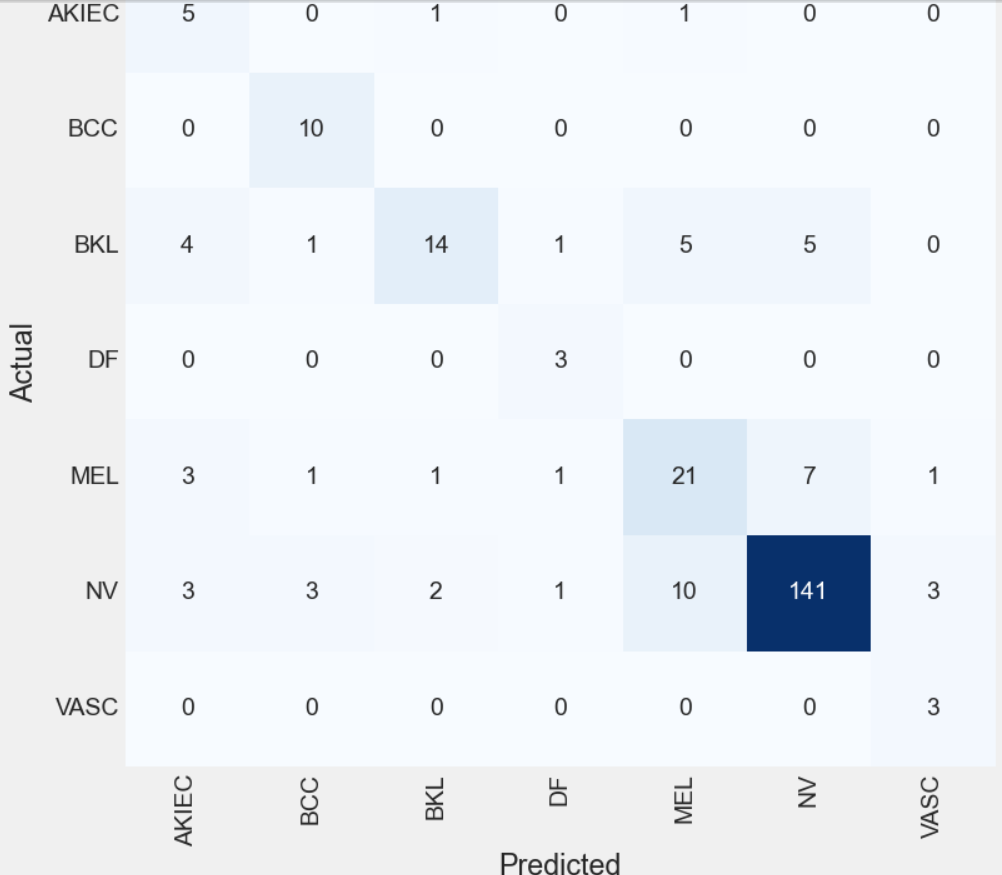
\includegraphics[width=0.45\textwidth]{./Graphics/confussion_matrix.png}
		\caption{Estadísticas de eficacia del modelo al estimar los resultados en el conjunto de pruebas.\label{fig:confussion_matrix}}
		\end{center}
		\end{figure}
    
    

%-----------------------------------------------------------------------------------
	\subsection{Estadísticas de aprendizaje}\label{sub:learning_statistics}
%-----------------------------------------------------------------------------------
		\begin{figure}[ht]%
      \begin{center}
      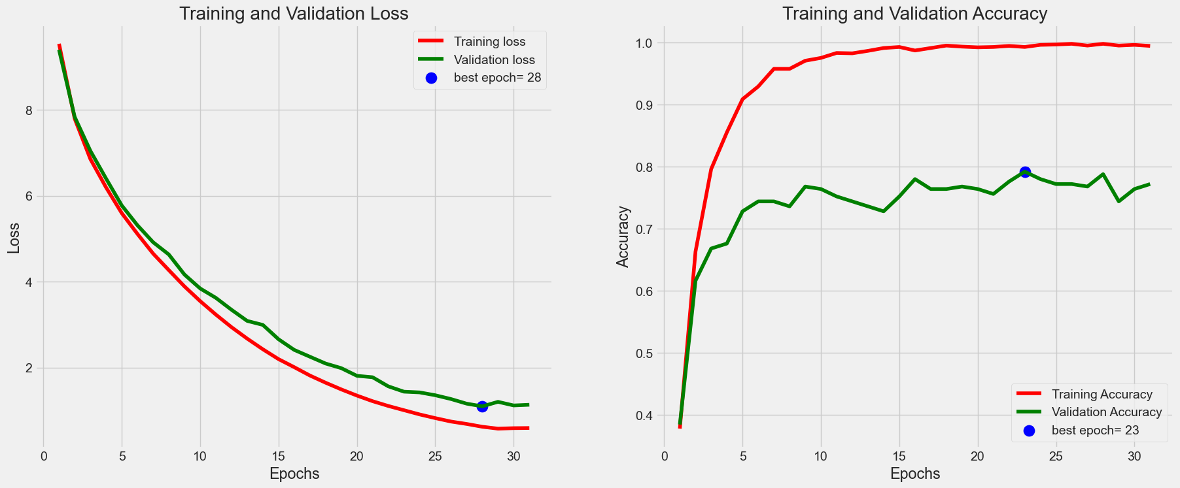
\includegraphics[width=0.45\textwidth]{./Graphics/training_validation.png}
      \caption{Estadísticas de aprendizaje a lo largo del proceso de entrenamiento (en rojo el proceso de entrenamiento en el conjunto de entrenamiento, en verde en el conjunto de validación).\label{fig:training_validation_loss}}
      \end{center}
		\end{figure}
  
La imagen anterior muestra un gráfico del curso temporal de las épocas realizadas, mostrando cómo el algoritmo iba obteniendo resultados más precisos y disminuyendo el error.

%-----------------------------------------------------------------------------------
\section{Ventajas y Desventajas}\label{sec:advantages_disadvantages}
%-----------------------------------------------------------------------------------
Las ventajas y desventajas del proceso son las siguientes. 
Ventajas: 
\begin{enumerate}
   \item Selección y representación del problema y de los datos. 
   Este proceso ayuda a comprender mejor el problema en cuestión y a identificar los datos relevantes necesarios para entrenar el modelo.
   \item Preprocesamiento de datos e imágenes. 
   Eliminar el ruido y los artefactos de las imágenes mejora la calidad de los datos y puede mejorar el rendimiento del modelo. 
   La selección de canales adecuados y la reducción del ruido también pueden mejorar el rendimiento del modelo
\end{enumerate}  
Desventajas: 	
\begin{enumerate}
   \item Modificación y procesamiento de datos. Si se utilizan conjuntos de datos inadecuados o se normalizan incorrectamente, el modelo puede no ser preciso o útil.
\end{enumerate} 

